\subsection{SHAP and LIME Visualisation}
Figure~\ref{fig:xai-global} summarises the 20 sampled held-out explanations from the tuned logistic models. The largest mean absolute SHAP contributions were associated with the source fields \texttt{bm} (0.208), CRP (0.173), extracellular-fluid/total-body-water ratio (0.071), vitamin D (0.068), weight (0.065), and extracellular water (0.056). The ordering describes this small sample and the fold-specific models, rather than a population-level ranking. Higher recorded CRP values generally contributed towards the absent class within these fitted models; this association does not imply a protective biological effect.

\begin{figure}[tbp]
\centering
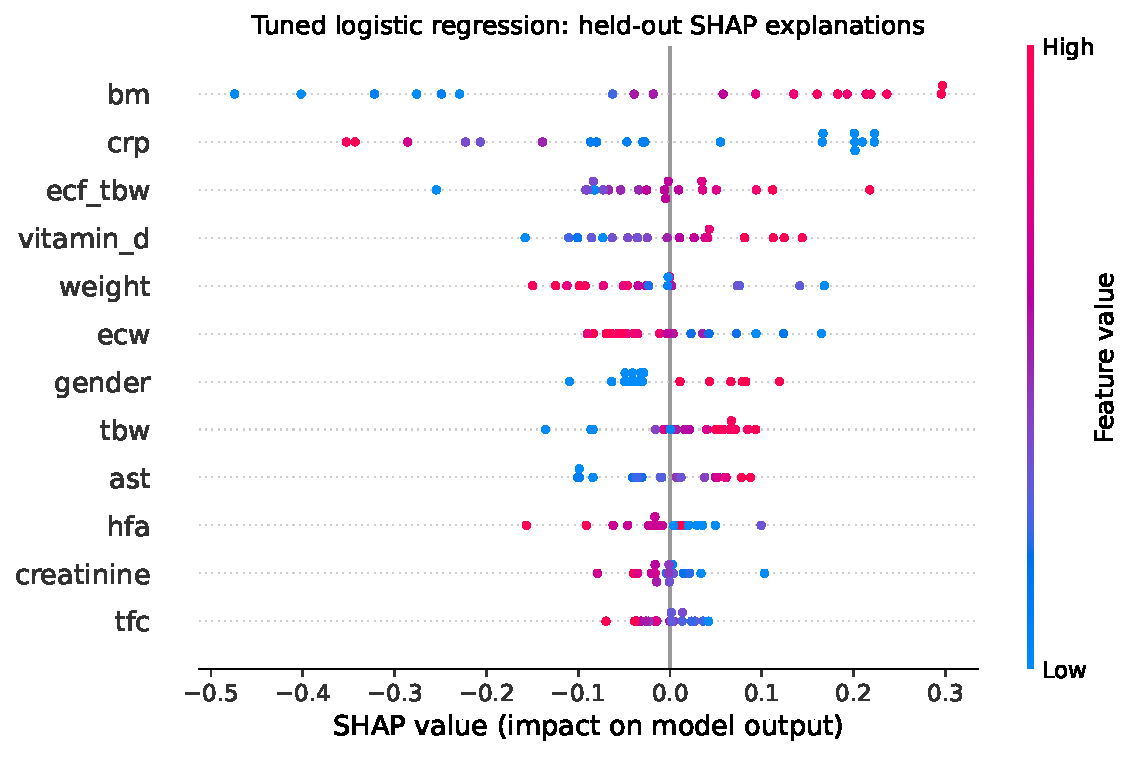
\includegraphics[width=0.88\linewidth]{figures/xai/global_shap.pdf}
\caption{Kernel SHAP summary for 20 sampled excluded records from tuned logistic Leave One Patient Out models. Each point uses its own outer-fold model and training-only background. Positive values increase the predicted probability of gallstones; negative values decrease it. Colour indicates the recorded feature value, and source-field labels follow the dataset schema. Features are ordered by sampled mean absolute contribution.}
\label{fig:xai-global}
\end{figure}

Figure~\ref{fig:xai-errors} compares SHAP and LIME for two confident errors. Source record 156 was a false negative with predicted probability 0.038; its largest displayed negative SHAP contributions included fluid ratio, \texttt{bm}, and vitamin D. Source record 178 was a false positive with predicted probability 0.995. These examples illustrate how multiple contributions can support an incorrect prediction despite aggregate discrimination. SHAP baselines were 0.443 and 0.413, respectively, and reconstruction from all feature contributions matched the saved probabilities. Only the eight largest contributions are displayed locally.

LIME surrogate $R^2$ was 0.423 for the false negative and 0.230 for the false positive, indicating limited local fidelity. For record 156, the surrogate prediction (0.160) also differed from the classifier probability (0.038). LIME condition weights and SHAP probability contributions have different meanings and should not be compared numerically. Agreement in direction is descriptive; correlated measurements and synthetic perturbations can produce unstable or implausible neighbourhoods.

\begin{figure}[p]
\centering
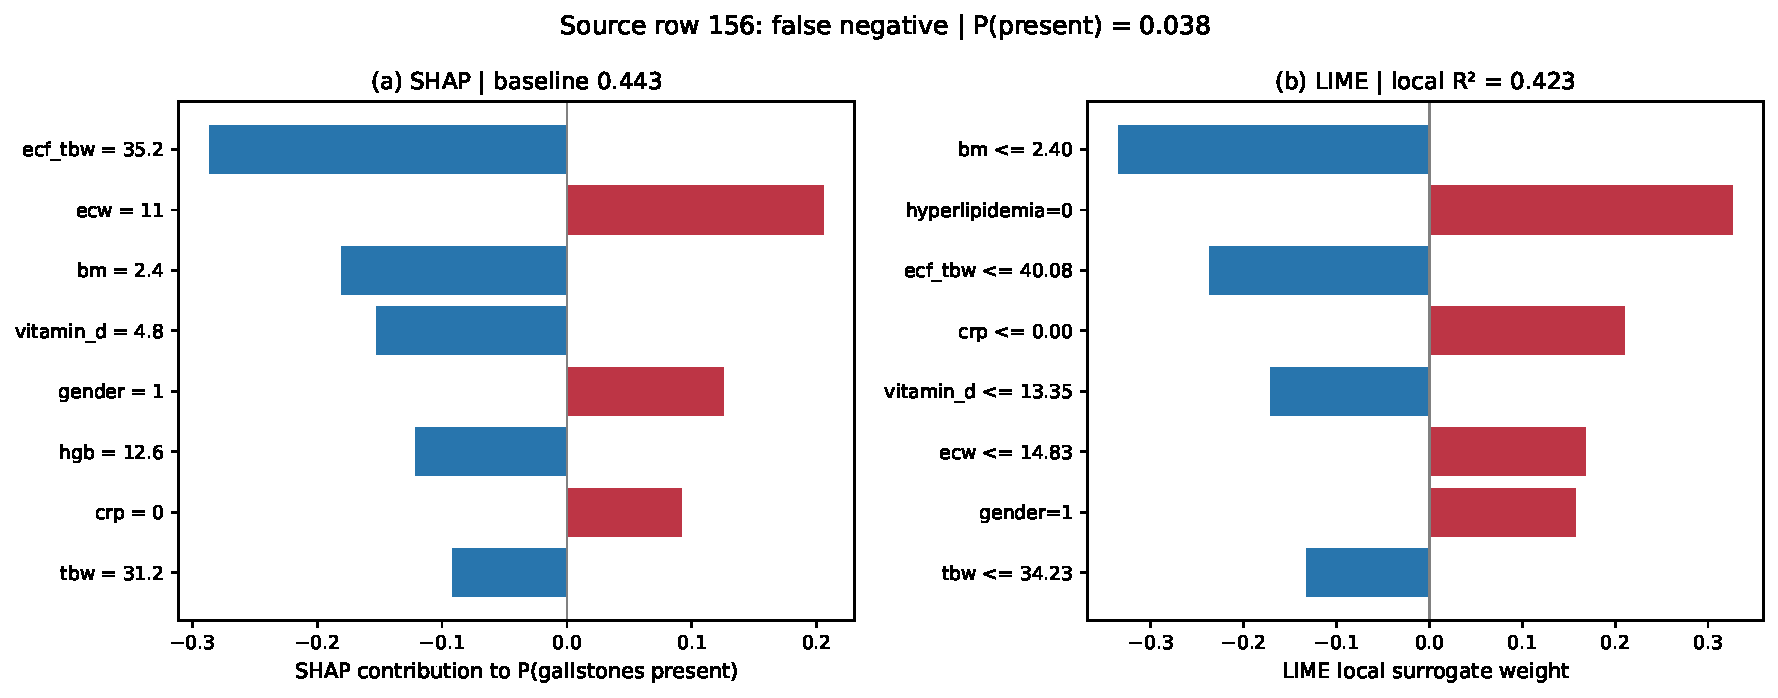
\includegraphics[width=\linewidth]{figures/xai/local_fn.pdf}
\par\medskip
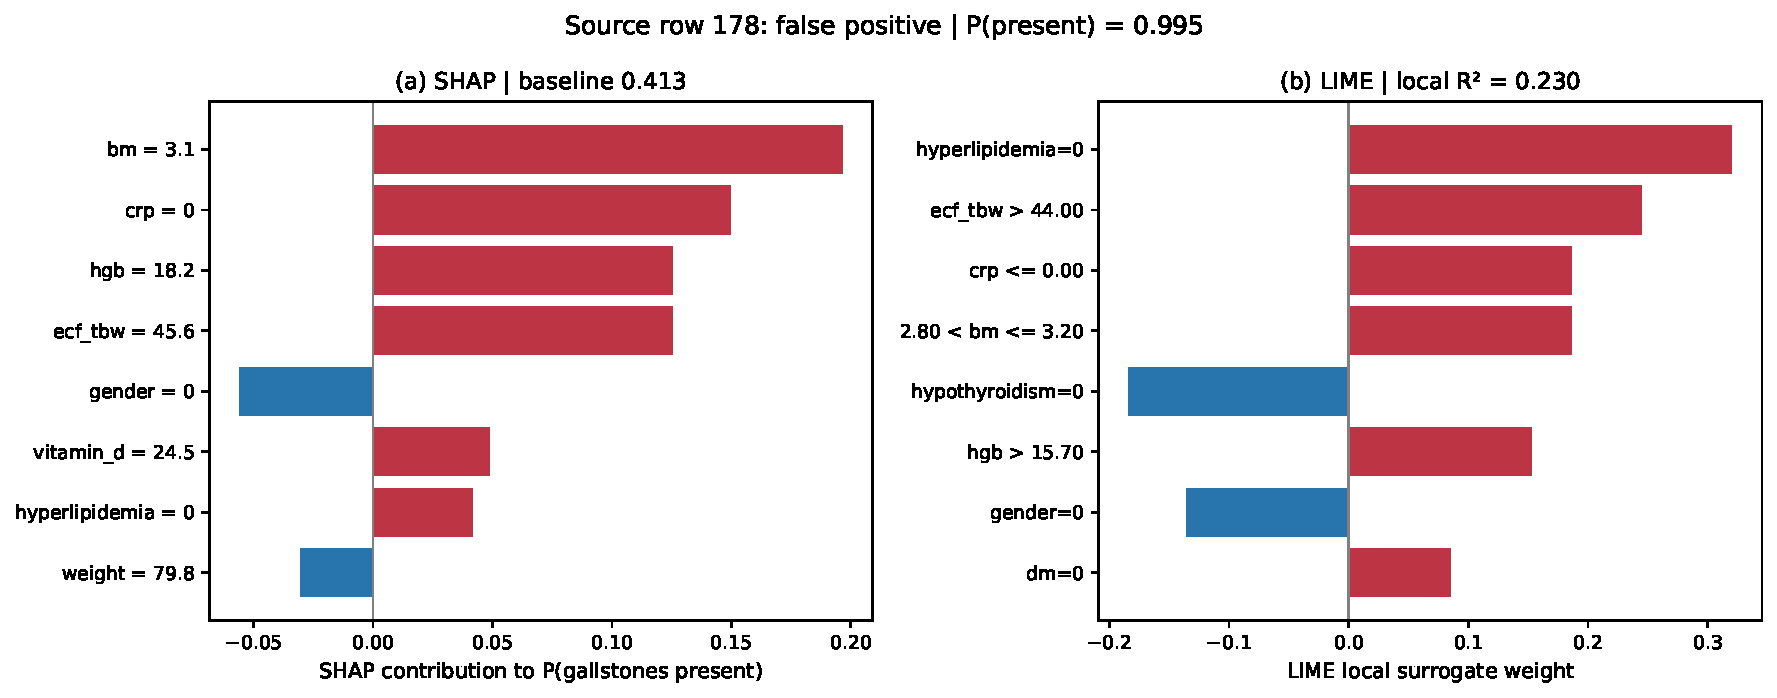
\includegraphics[width=\linewidth]{figures/xai/local_fp.pdf}
\caption{Local explanations of a retrospectively selected false negative (source row 156, top) and false positive (source row 178, bottom) from tuned logistic Leave One Patient Out evaluation. Left: the eight largest absolute SHAP contributions, labelled with recorded input values. Right: LIME condition weights and local surrogate fidelity. Red pushes towards gallstones present; blue pushes towards absent. Each excluded record was omitted from fitting, tuning, and explainer background construction. These selected examples do not estimate error prevalence.}
\label{fig:xai-errors}
\end{figure}
